\subsubsection{Chua's Circuit}
 \begin{itemize}
  \item \textbf{Methodology}
We constructed the circuit using 4 TL082 I.C.'s and commercial resistors with the values used during simulation, Trimmer resistors to be able to move the resistor values of R.

            \begin{figure}[h]
            \centering
            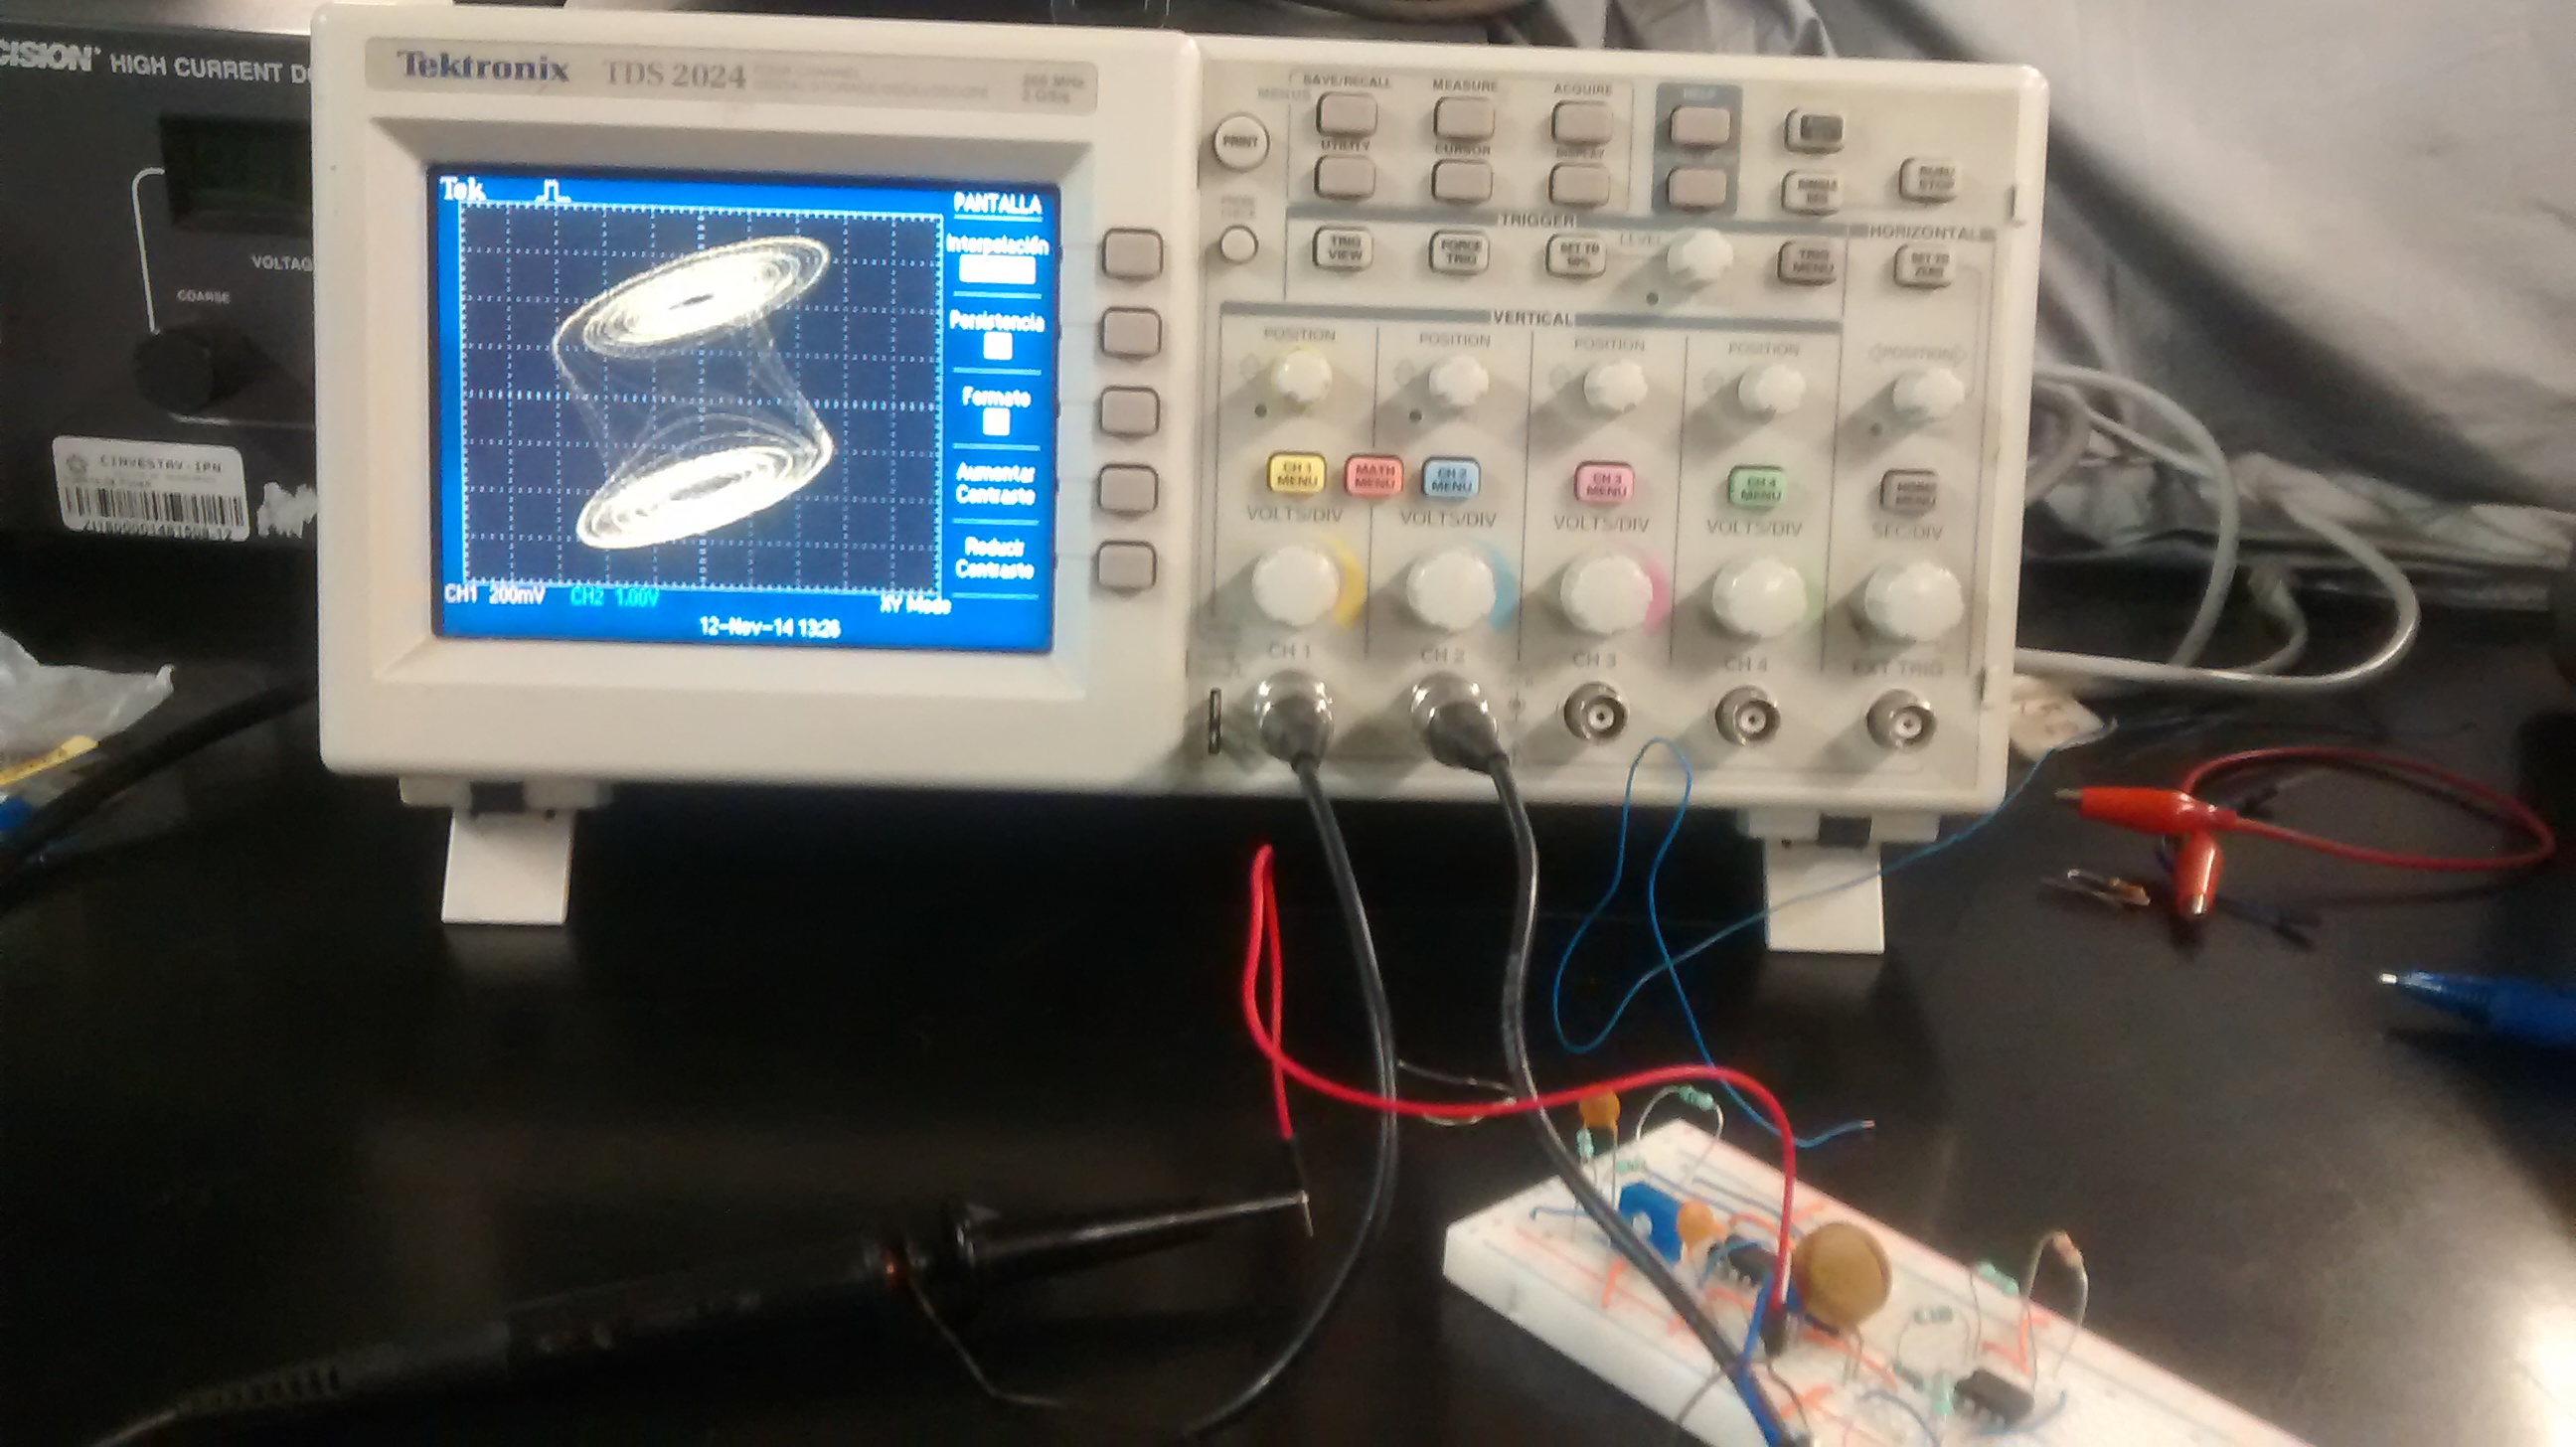
\includegraphics[scale=0.1]{imagenes/2-benford/chua_breadboard.jpg}
            \caption{Chua's System Breadboard}
            \end{figure}
We used two oscilloscope probes to measure the voltage from the two capacitors, and did our measurements with  a Tektronix DS201 Oscilloscope with a direct method sampling.

 The first digit distribution was determined from the voltage measured at the terminals of C1,varying R from 1700$\Omega$ to 1900$\Omega$in $25\Omega$ intervals, values in which Chua's Circuit presented chaotic behaviour. The first digits (without leading zeroes) of the voltage values at discrete points were analyzed, the oscilloscoped allowed us to take 2000 samples from a 250 $\mu$s period. We compared the first digit distribution of the dataset with the distribution given by Benford's Law using the Mean Absolute Deviation (MAD) proposed by \cite{Nigrini97}.



  \item \textbf{Results}
We put a table with the MAD results at each value of R:
\begin{center}
  \begin{tabular}{ c | c | c }
R & VC1 & VC2\\
1700 & 0.0265740826252 &0.0941252615083\\ \hline
1725 &  0.0308583854254& 0.0894910362566\\ \hline
1750 & 0.0225012003889 & 0.0937811348396\\ \hline
1775 &  0.0213932963068 & 0.0894482136018\\ \hline
1800 &  0.0515553953624& 0.0817178075546\\ \hline
1825 & 0.0620516456615 &0.0757908400412\\ \hline
1850& 0.0801858066881 &0.0616474503737\\ \hline
1875 & 0.0864648516751& 0.0566898036332\\ \hline
1900 &0.0848654579991 &0.0477795566486\\ \hline


  \end{tabular}
\end{center}

The closest value we got was with R=1775 measuring VC1
            \begin{figure}[h]
            \centering
            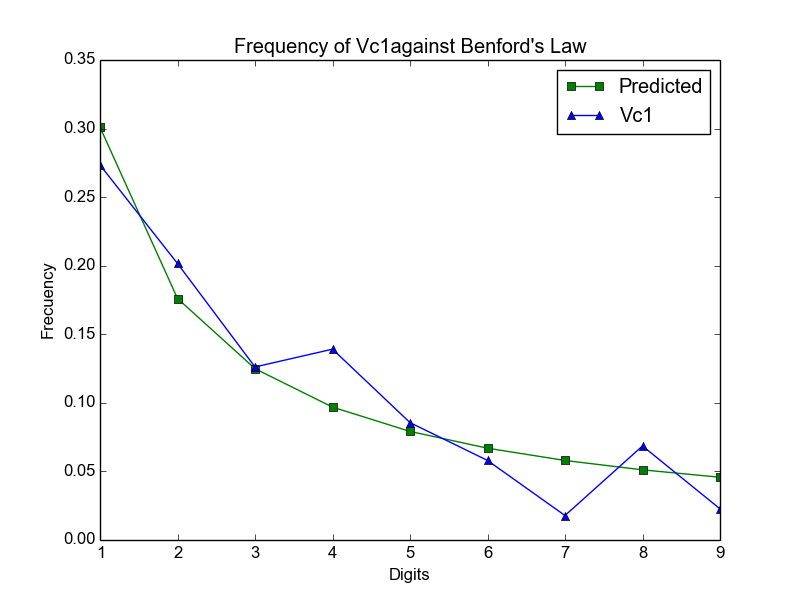
\includegraphics[scale=0.4]{imagenes/2-benford/benford_chua1775.png}
            \caption{Benford's Law against VC1}
            \end{figure}
  \item \textbf{Remarks}

We noticed that between for R between 1730 and 1775, there is a more clear First Digit Distribution according to Benford's Law, however, the measurements did not comply with MAD's Criteria which expects at most 0.015 in order to be compliant with Benford's Law. We also took a measurement with R=2000$\Omega$, value at which the system behaves as a quasi-periodic oscillator. we noticed that the first digit distribution is more uniform.

\begin{figure}
         \centering
            \begin{subfigure}[b]{0.4\textwidth}
            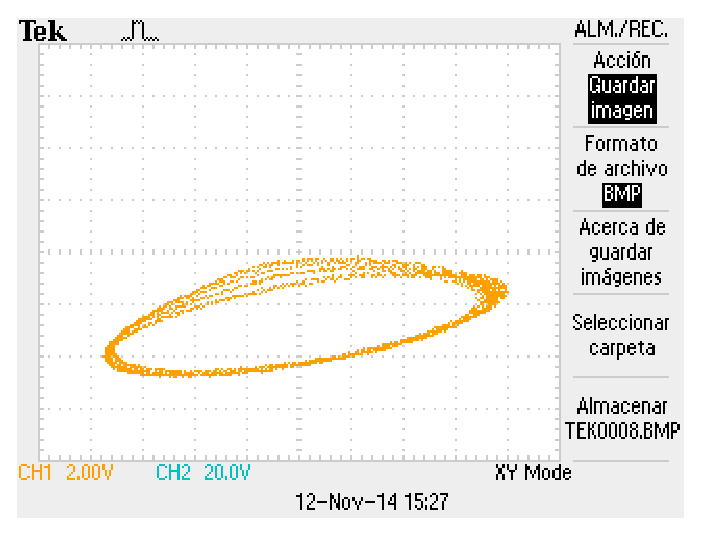
\includegraphics[width=\textwidth]{imagenes/2-benford/chua_2000.eps}
            \caption{V1-V2 $V_x$ vs $V_y$ plot}
            \end{subfigure}
            \begin{subfigure}[b]{0.8\textwidth}
            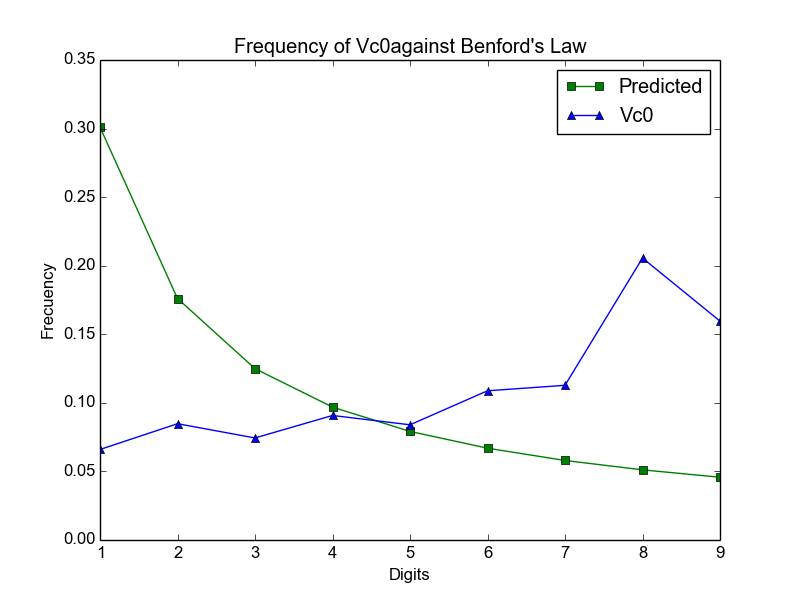
\includegraphics[width=\textwidth]{imagenes/2-benford/benford_chua20.png}
            \caption{Bifurcation Diagram varying b}
            \end{subfigure}
\end{figure}

 \end{itemize}
\subsubsection{Takougang Circuit}
 \begin{itemize}
  \item \textbf{Methodology}The circuit was connected using a standard breadboard, according to the diagram, all passive components had a nominal value equal to the ones proposed in the schematic, with a tolerance of 5\%. A regulated voltage source, set to $\pm$ 12 V was utilized to feed the active components which were the same as stated in the schematic. A third output of the regulated voltage source served to provide a stable input for the circuit ($V_b$). Next, a digital oscilloscope was used in order to obtain the data provided by the circuit.

A 1 GHz band-width oscilloscope (Agilent DSO6104A) was used next, and it was configured in order to reduce random noise. The sampler uses an averaging algorithm which delivers data with less noise, and reduces the vertical resolution (as low as 0.7 mV), with the data obtained from that oscilloscope the analysis was more reliable and results confirmed what was expected from the simulations, although only 1000 samples in an interval of 10 ms were fetched.
  \item \textbf{Results}
The first digit distribution of the voltages was taken and following the same methodology as with Chua's System, we swept through $V_b$ and took the MAD value from each distribution
\begin{center}
  \begin{tabular}{ c | c | c }
    \hline
$V_b$  & $V_x$&$V_y$\\ \hline
82mV & 0.0775279989288 & 0.0607280417648 \\ \hline
92mV & 0.0789296997697 &  0.0620760330126 \\ \hline
102mv & 0.0779822062934 & 0.0620098514762  \\ \hline
112mv & 0.0722551588234 & 0.0586329019652  \\ \hline
117mv & 0.0731369417692 & 0.0565637073089  \\ \hline
122mv & 0.0761361923841 & 0.0607646781498  \\ \hline
127mv & 0.0702382876578 & 0.0581541345311  \\ \hline
132mv & 0.0726371865346 & 0.0568562424256  \\ \hline
137mv & 0.0723923763659 & 0.0588608733569  \\ \hline
142mv & 0.0689722218274 & 0.0566979795649  \\ \hline
147mv & 0.0649140903028 & 0.0492049220995  \\ \hline
152mv & 0.0689575397758 & 0.0540809650999  \\ \hline
157mv &0.071269709088 & 0.0556102788266   \\ \hline
167mv &0.0713877270204 & 0.0546276659144  \\ \hline
187mv & 0.0642837364043 & 0.0499581746439  \\ \hline
197mv &0.0619961498144 & 0.0491763886427  \\ \hline
217mv & 0.0644054740322 & 0.0521147934116  \\ \hline
237mv & 0.0574813303354 & 0.0515391121266  \\ \hline
257mv & 0.0552768884655 & 0.0514296383228  \\ \hline
277mv & 0.0464325092508 & 0.0450451557158  \\ \hline
112mv (H-Res) &0.0126362748635 & 0.0149581584175  \\ \hline
132mv  (H-Res)& 0.0114562387312 & 0.0056682935093  \\ \hline
152mv  (H-Res)& 0.0106402668795 & 0.0143777130129  \\ \hline
172mv  (H-Res)& 0.0077090293797 & 0.0118696485616  \\ \hline
192mv  (H-Res)& 0.00801241025011 & 0.0120739312228  \\ \hline

  \end{tabular}
  \end{center}

We notice we have the best agreement with Benford's Law with $V_b=132mV$ Which gives a MAD value of 0.0056

            \begin{figure}[h]
            \centering
            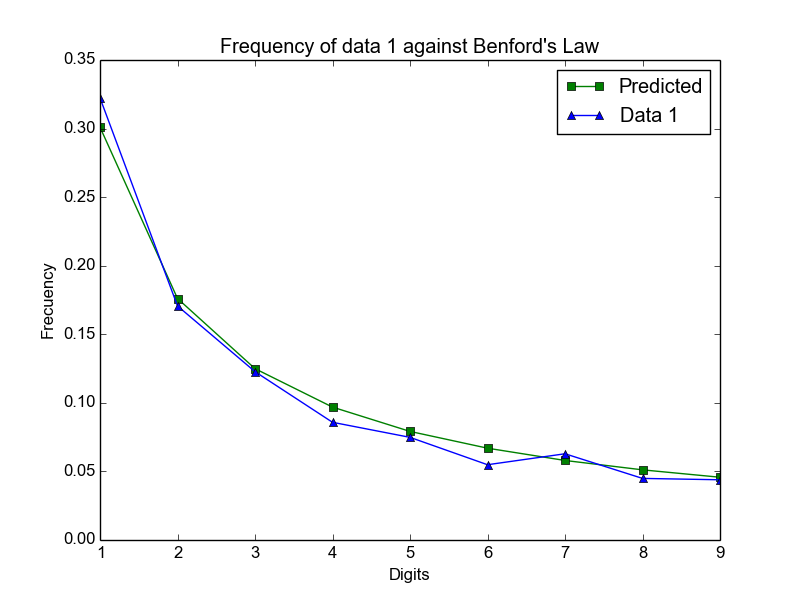
\includegraphics[scale=0.4]{imagenes/2-benford/benford_shilnikov_1.png}
            \caption{Benford's Law against digit distribution of $V_y$}
            \end{figure}

  \item \textbf{Remarks}

Simulations from Simulink gave a better accordance with $V_b=132mV$, however measuring without High-resolution sampling we did not obtain proper distributions, until we activated that sampling method, we got a distribution according to Benford's Law
 \end{itemize}
